\subsection{From Intuition to Examples}

    
    \emph{Any reads-from relation between a read (r) and a write (w) will be written as \textbf{r:w}} 


    \paragraph{Examples to show Write orders important}

        The following two examples show why having a symmetric order between same writes of each equal thread is important. 
        \begin{figure}[H]
            \centering 
            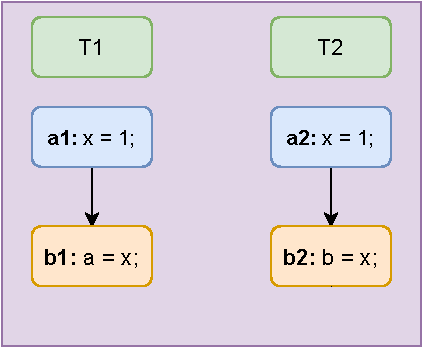
\includegraphics[scale=0.7]{Example1(2+wr).pdf}
            \caption{2+wr}
        \end{figure}

        The above example has the following possibilities of read-write relations that result due to an execution. Note that $b1:a2 , b2:a1$ is not possible due to coherence being our assumption. 
        \begin{align*}
            b1:a1 , b2:a1 \\ 
            b1:a1 , b2:a2 \\
            b1:a2 , b2:a2
        \end{align*}

        Observations:
        \begin{itemize}
            \item $b1:a1, b2:a1$ implies an ordering on the writes such that $a2$ occurs before $a1$.
            \item $b1:a2, b2:a2$ implies an ordering on the writes such that $a1$ occurs before $a2$.
            \item The above two executions are symmetric to each other as we can swap threads of one to get the other. 
            \item We need to fix an ordering between the equal writes of symmetric threads. 
        \end{itemize}
    
        \begin{figure}[H]
            \centering 
            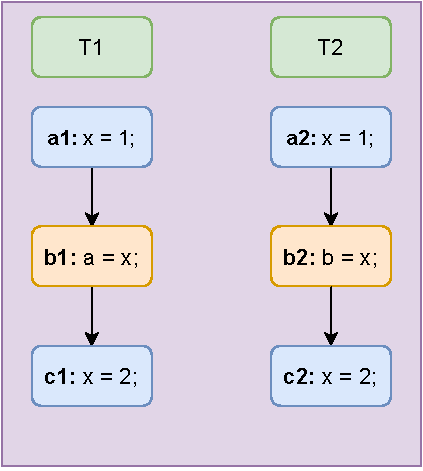
\includegraphics[scale=0.7]{Example2(2+wrw).pdf}
            \caption{2+wrw}
        \end{figure}
        
        The above example is an extension of the previous, by adding two writes following the reads to the same memory. Note that the outcome $b1:c2, b2:c1$ is not considered due to lack of Load-Buffering (I still think its Coherence). The following are the possible executions in terms of read-write relations. 

        \begin{align*} 
            b1:a1 , b2:a2 \\
            b1:a1 , b2:c1 \\ 
            b1:a2 , b2:a2 \\
            b1:a2 , b2:c1 \\
        \end{align*}

        Observations:
        \begin{itemize}
            \item $b1:c2, b2:a2$ is not counted as it implies that $c2$ is before $c1$, whose reverse is already covered by $b1:a1 , b2:c1$
            \item Same argument for why the case $b1:c2, b2:a1$ is not considered.
            \item A slight hint is given that ordering between reads also matters. (the case $b1:c2, b2:a2$ also implies $b2$ occurs before $b1$.) 
        \end{itemize}

    \paragraph{Examples to show Read Orders are(or may be) not important}

        \begin{figure}[H]
            \centering 
            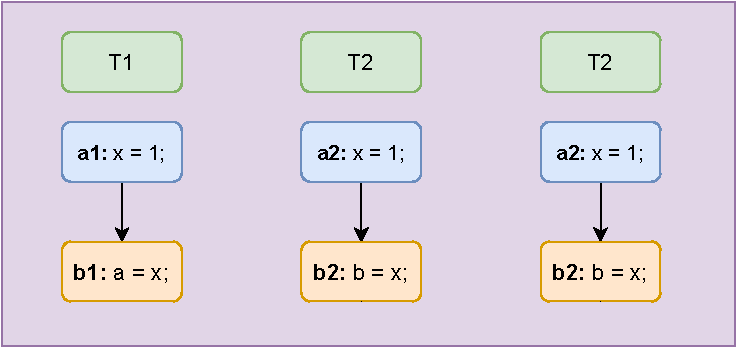
\includegraphics[scale=0.7]{Example3(3+wr).pdf}
            \caption{3+wr}
        \end{figure}


        The above example is extending the first example with another symmetric thread. It has the following executions covered using our insight from the previous examples. 
        \begin{align*}
            b1:a1 , b2:a2 , b3:a3 \\
            b1:a1 , b2:a3 , b3:a3 \\
            b1:a2 , b2:a2 , b3:a3 \\
            b1:a2 , b2:a3 , b3:a3 \\
            b1:a3 , b2:a2 , b3:a3 \\
            b1:a3 , b2:a3 , b3:a3
        \end{align*}

        Observation:
        \begin{itemize}
            \item $b1:a1 , b2:a3 , b3:a3$ and $b1:a2 , b2:a2 , b3:a3$ appear to be symmetric, but considering the total order between equal writes also as part of execution, they are not symmetric, rather they are unique. 
            \item  $b1:a3 , b2:a2 , b3:a3$ is a case we would not have covered, if we enforced an order between reads, as it would then mean that $b2$ can only read from $a3$. 
            \item Enforcing read orders prevent the above case. The above case is valid because $b2:a2$ implies no ordering between writes, hence the order between $a1$ and $a2$ can be left to us. 
            \item \textcolor{red}{However, the above case is symmetric to $b1:a2 , b2:a2 , b3:a3$; swap identities of thread $T2$ and $T3$}
            \item This strengthens our intuition of equivalent executions that can be obtained by swapping thread identities, due to reversing implied orders between writes. 
        \end{itemize}

        \critic{red}{Not enforcing an order between reads, may have issues about completeness, meaning we might cover a few redundant explorations.}

        \begin{figure}[H]
            \centering
            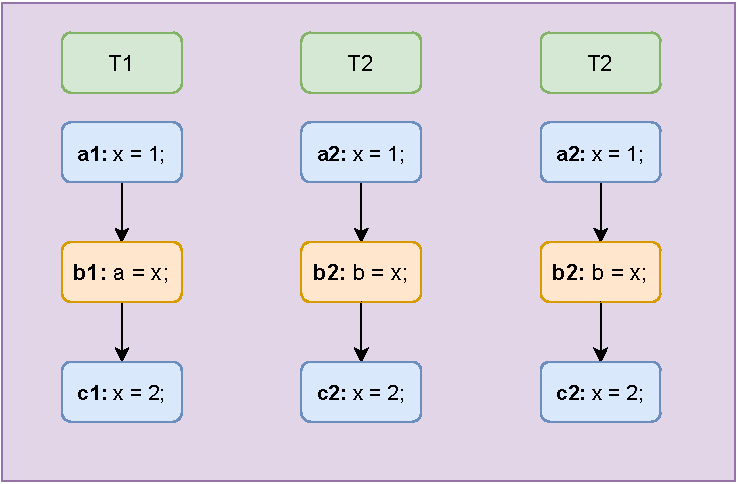
\includegraphics[scale=0.7]{Example4(3+wrw).pdf}
            \caption{3+wrw}
        \end{figure}

        The above example is extending the previous with additional writes to each thread. The possible executions are many, hence not all of them will be elicited, but ones of focus: 
        
        \begin{align*}
            b1:a1 , b2:a3 , b3:c1 \\
            b1:a3 , b2:a2 , b3:c2 \\
            b1:a1 , b2:a2 , b3:c1 \\
            b1:a2 , b2:a2 , b3:c1 \\
        \end{align*}

        Observation:
        \begin{itemize}
            \item $b1:a1 , b2:a3 , b3:c1$ would not be explored if we consider $b1:a1 , b2:a3 , b3:a3$ to be symmetric to $b1:a2 , b2:a2 , b3:a3$. Considering them symmetric would make us assume that when $b1:a1$, then $b2$ cannot read from any outside write other than that of $T1$. 
            \item $b1:a3 , b2:a2 , b3:c2$ would not be explored if we ordered the reads too. However, it is also the case that $b1:a1 , b2:a3 , b3:c1$ is symmetric to this (just swap thread identities of $T1$ and $T2$). Further investigation is needed. This tells our approach may not be complete. 
            \item \textcolor{red}{$b1:a1 , b2:a2 , b3:c1$ is symmetric to $b1:a1 , b2:a2 , b3:c2$ , but it does not violate our requirement of implied write orders.}
            \item \textcolor{red}{$b1:a2 , b2:a2 , b3:c1$ is symmetric to $b1:a3, b3:a3, b2:c1$, but it does not violate our requirement of implied write orders.} 
            \item Conclusion from this example is that implied write orders is not complete. 
        \end{itemize}

        
    \paragraph{Examples to show affects of external non-symmetric writes}
        %Now consider extending the first example with another non symmetric thread 2+wr+w
        \begin{figure}[H]
            \centering 
            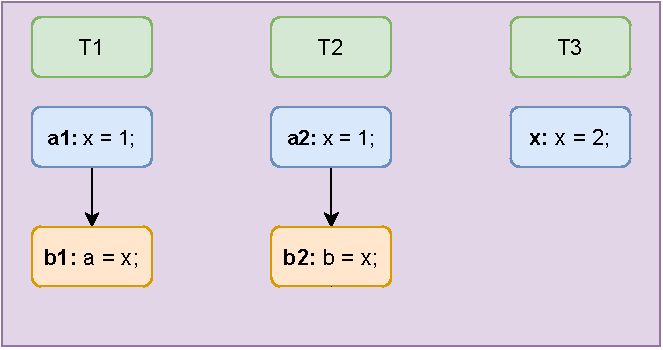
\includegraphics[scale=0.7]{Example5(2+wr+w).pdf}
            \caption{2+wr+w}
        \end{figure}

        The above example is the first program extended with another non-symmetric thread having a write to same memory. We elicit the following possible executions, catering to our rules for implied write orders: 
        \begin{align*}
            b1:a1 , b2:a2 \\
            b1:a1 , b2:x \\
            b1:a2 , b2:a2 \\
            b1:a2 , b2:x \\
            b1:x , b2:x \\
            b1:x , b2:a2
        \end{align*}

        Observations: 
        \begin{itemize}
            \item There is no restriction on order with the write $x$ and $a1, a2$.
            \item $b1:x , b2:a2$ is symmetric to $b1:a1 , b2:x$. But both of these explored do not violate implied write orders. 
            \item $b1:x , b2:a2$ can correspond to an order of writes being $a1->x->a2$ still respecting the order of writes that must hold. Whereas, $b1:a1 , b2:x$ can correspond to the order of writes being $a1->a2->x$ also respecting the order of writes that must hold. 
        \end{itemize}

        \begin{figure}
            \centering
            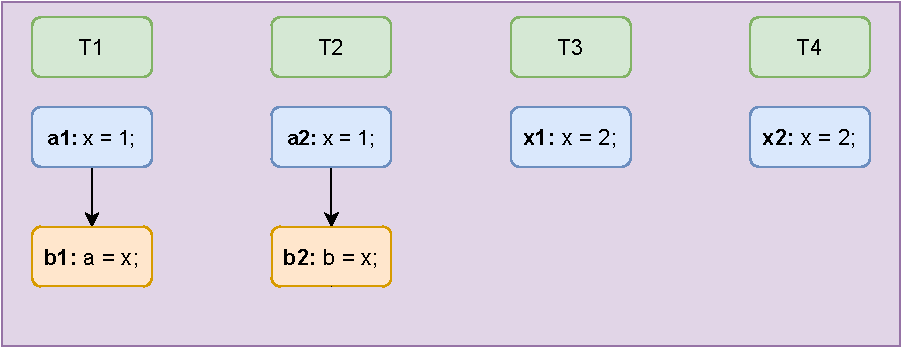
\includegraphics[scale=0.7]{Example6(2+wr+2+w).pdf}
        \end{figure}

       
        The above example is with two symmetric sets of threads. We have the following executions possible keeping our implied writes rule intact. 

        \begin{align*}
            b1:a1 , b2:a2 \\
            b1:a1 , b2:x1 \\
            b1:a1 , b2:x2 \\
            b1:a2 , b2:a2 \\
            b1:a2 , b2:x1 \\
            b1:a2 , b2:x2 \\
            b1:x1 , b2:a2 \\
            b1:x1 , b2:x2 \\ 
            b1:x2 , b2:a2 \\
            b1:x2 , b2:x2 \\
            b1:x2 , b2:x1
        \end{align*}

        Observation:
        \begin{itemize}
            \item \textcolor{red}{$b1:x1 , b2:x2$ is symmetric to $b1:x2 , b2:x1$, yet these two do not violate the implied writes.} rules. 
        \end{itemize}
        
        Notice that we do not have the case $b1:x2 , b2:x1$, as it implicitly violates the ordering constraint that $b1$ occurs before $b2$.

        (Still ongoing, examples with operations to multiple memory segments need to be analyzed)

        %Lastly consider the case 3+wrw+w

        %Keep this section open to more interesting examples